This chapter addresses the software architecture.
It starts by generating audio test files. Then, it configures the firmware to allow execution of \textit{TwoLAME} encoding algorithm. Afterward, basic software optimizations are done in the system. In the end, profiling analysis defines which part of \textit{TwoLAME}'s algorithm requires hardware acceleration.

Before being ported to the IOb-MP2-E, the \textit{TwoLAME} software was tested in a Linux~\cite{bib:gnulinux} environment, allowing one to verify its functionality independently before integration. This verification had a rudimentary character since the \textit{TwoLAME} software had already been tested and approved by a wide range of users in various systems. Therefore, the verification consisted of listening to both an original audio file and the corresponding encoded file, produced by \textit{TwoLAME}.

\subsection{Audio test files}

In this context, \textit{Audacity} software~\cite{bib:audacity} was used to generate four audio files. This free open-source software, compatible with multiple operating systems, is capable of multi-track audio editing and recording. 
The creation of multiple testing files was less about functionality verification and more about preparing for the algorithm's testing in the upcoming phases of this work, motivated by the following ideas:

\begin{itemize}

    \item \textbf{Variation in Audio Characteristics}: Testing files with diverse audio characteristics, including codec variations, encoding settings, and audio durations, allow a comprehensive assessment of \textit{TwoLAME}'s adaptability.
    \item \textbf{Consistency Across Specifications}: Maintaining consistent software performance across various specifications is crucial for a real-time encoding IP core. Using multiple test files ensures that \textit{TwoLAME} handles diverse audio sources, guaranteeing reliable real-time encoding performance regardless of input variations.
\end{itemize}

The first generated file was \textit{short.wav}, using the \textit{Generate Tone} option in \textit{Audacity}. This mono audio has a sine waveform, 44.1kHz sampling rate, 16 bits per sample, and a size of 27KB (the smallest audio file in the repository). 
The second generated file was \textit{long.wav}, using the \textit{Generate Rhythm Track} option configured with \textit{Metronome Tick} beat sound in \textit{Audacity}. This mono audio has a 44.1kHz sampling rate, 16 bits per sample, and a size of 683KB. 
The third generated file was \textit{noise.wav}, using the \textit{Generate Noise} option configured with \textit{White} noise type in \textit{Audacity}. This audio has a 44.1kHz sampling rate, 16 bits per sample, a size of 529KB and, unlike the previous ones, it is stereo. The mono default track was duplicated, with one being distributed 100\% to the Left and the other being distributed 100\% to the Right (\textit{panning effect}). 
The fourth and last generated file was \textit{vivaldi.wav}. This file was not generated from scratch in \textit{Audacity}. Instead, it was simply converted to WAV format. The original file, entitled 'Vivaldi - Spring', was downloaded from the Internet (for free) and opened on \textit{Audacity}. After that, the track was reduced to the initial 4 seconds and exported as WAV, being also stereo. What motivated the use of this file was the recognized quality and complexity of \textit{Vivaldi}'s songs~\cite{vivaldi}.
Testing with both mono and stereo files is crucial for assessing versatility and performance across various scenarios. Mono files are valuable for evaluating bandwidth efficiency and compatibility with single-channel content, while stereo files help assess the encoder's ability to preserve spatial characteristics and deliver an immersive listening experience.

At this point, it was already possible to verify the \textit{TwoLAME} software using the audio files available at the repository. From a standard \textit{automake} process, composed of \textit{./configure}, \textit{make}, and \textit{make install} commands, \textit{TwoLAME} was successfully installed in the environment. Then, by simply executing \textit{./stwolame} followed by the input file name and the output file name (the one desired), the software would run and produce an MP2 version of the original file. 
In the process, both input and output file names should include the file extension. By executing the \textit{stwolame short.wav short.mp2} command, it was verified that both the original and the encoded audio files sounded the same (for a human listener). The same happened with the second and fourth files through a similar command. 
The third file is not audible, in the way that it was created just to verify proper correctness in terms of values produced by the system (in upcoming phases). This is because white noise is the worst-case scenario for audio encoding, mainly due to its high requirements. 

With the original \textit{TwoLAME} software verified, the next step was porting \textit{libtwolame} (\textit{TwoLAME}'s library) to the IOb-MP2-E, which required a front-end interface.

\subsection{Firmware}

Based on the \textit{simplefrontend} example present in \textit{TwoLAME}'s repository, the front end was implemented in \textit{firmware.c}. As the name indicates, this file specifies the firmware through some C code. More precisely, it specifies the firmware that runs on the CPU as a software application which, in this work, is intended to be the \textit{TwoLAME} algorithm. To allow that, the firmware is converted into machine instructions that are specific to the RISC-V instruction set~\cite{bib:riscvmanual_iieec}, being interpreted by \textit{VEXRISCV} (more details in the \textit{Hardware architecture} section). 
Figure \ref{newpseudo} shows the pseudo code for the \textit{main()} function in \textit{firmware.c}.

\begin{figure}[H]
\centerline{\fbox{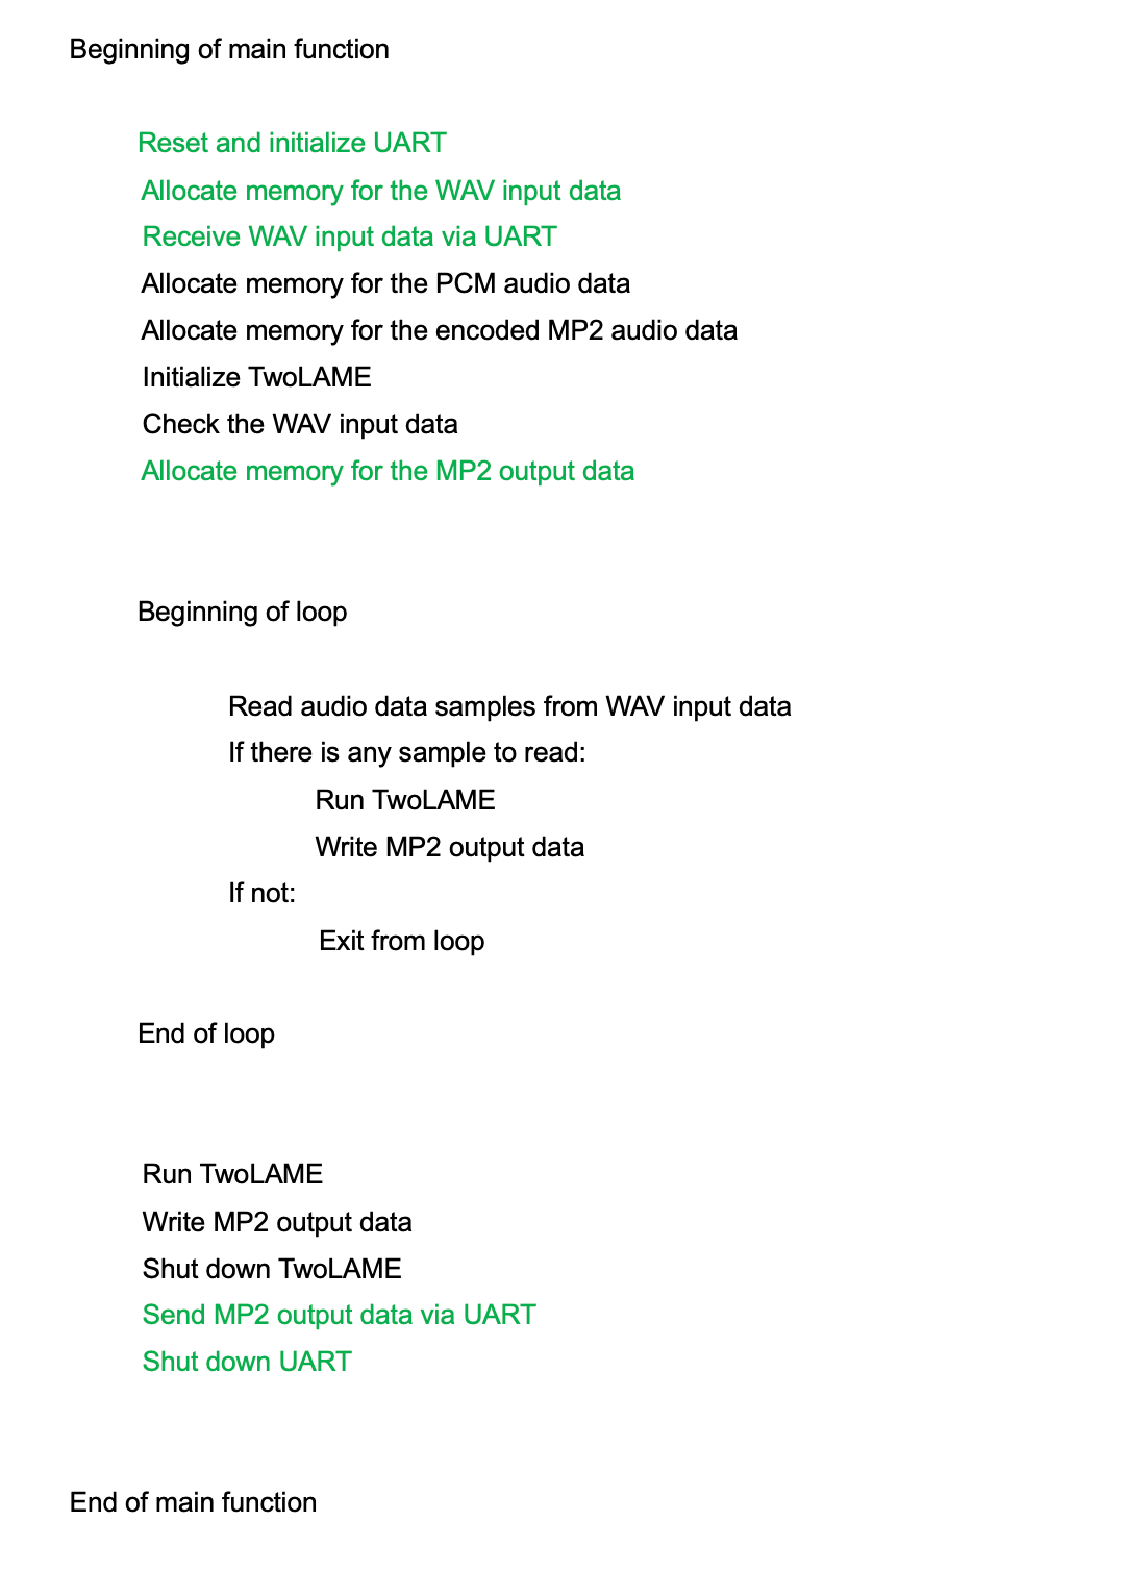
\includegraphics[width=0.80\linewidth]{newpseudo.pdf}}}
\caption{New \textit{firmware.c} pseudo code.}
\label{newpseudo}
\end{figure}

The first difference in \textit{main()} is the usage of \textit{uart\_init}, which resets \textit{IObundle, Lda}’s UART peripheral and sets its division factor. This peripheral is needed to transmit data to IOb-MP2-E's external memory via UART. 
There are also two additional memory allocations for the input and output data. These operations are done through \textit{malloc} using unsigned char type because the UART peripheral transmits one byte at a time.
After allocating memory, the input audio data is received via UART in \textit{uart\_recvfile}. The function receives the path as an argument, which is defined as \textit{test.wav}. This is a generic name since the input audio file is copied to the compiling directory as \textit{test.wav}.
The previous modifications were done as the IOb-MP2-E does not have an operating system or file system. For this reason, the \textit{fopen} function inside \textit{wave\_init} was removed. Furthermore, in each iteration of the \textit{while} loop, a chunk of input data is read from the input data using \textit{fread}. Since this function, present in \textit{wave\_get\_samples}, also requires a file system, there should be some process to increment the pointer to the input data, so that \textit{fread} can be removed. This is achieved by decrementing a global variable (unread\_data) based on the number of samples read in each loop iteration. In addition, since the \textit{pcmaudio} buffer should contain short integers, there is a process inside \textit{wave\_get\_samples} that converts every two characters into a single short integer. This is done by concatenating two characters, with the first one shifted left eight positions.

Nonetheless, not only the input audio data is received but also the output audio data is sent from IOb-MP2-E's external memory, both via UART. Thus, the \textit{fwrite} functions were also removed from \textit{main}.
More precisely, there was one situation inside the \textit{while} loop and another after the loop, with both \textit{memcpy} insertions being responsible for writing the MP2 output data, replacing \textit{fwrite} calls. An important detail about this modification comes with the pointer to the output data. Just like in \textit{wave\_get\_samples}, there should be a process to increment the pointer to the output data, so that the new data does not overwrite previous data. This process is based on the number of frames encoded in each loop iteration, specifically inside \textit{\textit{TwoLAME}\_encode\_buffer\_interleaved} function.
One of the last modifications in \textit{main} consists of sending the output data via UART in \textit{uart\_sendfile}. The function receives the path as an argument, which is defined as ’../../encoded.mp2’. This way, the output audio file is copied to the main repository directory as \textit{encoded.mp2}.
Afterward, the UART transmission is closed through \textit{uart\_finish}, and the program returns.

Apart from \textit{main}, some header files were included in \textit{firmware.c}, related to both the IOb-MP2-E system and \textit{libtwolame}. Two macros were also defined, AUDIOBUFSIZE as 2304 and MP2BUFSIZE as 4096. These variables specify the size of input and output buffers, respectively, which in practice represent the chunk of data encoded each time (the number of frames encoded). Therefore, the number of frames can be altered by changing both variables on the same scale. As it stands, the \textit{TwoLAME} encodes one frame at a time. 
After this process, the system was emulated on PC, passing through a simulation environment developed by \textit{IObundle, Lda}, which allowed full testing. 

\subsection{Optimization}

Regarding execution in FPGA, some basic software optimizations were performed.
According to what was previously stated about the use of \textit{VEXRISCV} CPU, the first change in \textit{libtwolame} was the software precision. In \textit{comon.h}, there is a macro for FLOAT that was initially defined as \textit{double}, but it was changed to \textit{float}. One reason for this is the fact that \textit{TwoLAME} should be faster rather than more accurate (single-precision is already much better than fixed-point), without compromising the encoded audio quality.
Apart from altering the macro, one function in \textit{subband.c} was also changed. The original code contained \textit{modf}~\cite{modf}, a function that belongs to \textit{math.h}~\cite{mathh} and requires double precision. Therefore, it was substituted by \textit{modff}~\cite{modf}, which has the same functionality (returns the fractional part) but uses single precision.

The second change was more strategic, as it entailed a meticulous analysis of the encoding software. It is well-established that trigonometric functions~\cite{trigonometric} are computationally intensive operations, particularly for audio-processing software like \textit{TwoLAME}. These functions, while mathematically accurate, can be computationally expensive and can slow down the encoding process. Therefore, a common practice in software engineering is to substitute this type of function with precomputed lookup tables, for specific input ranges. This allows the software to access and interpolate results much more quickly than it could by performing complex calculations on the fly. 
To evaluate this possibility, the \textit{TwoLAME} was emulated on PC using different input test files.

The first case was \textit{psycho\_3\_powerdensityspectrum}, in \textit{psycho\_3.c}. In this function, there was a \textit{log10} operation inside a \textit{i} loop, with \textit{i} ranging from 1 to 512 (HBLKSIZE-1). Since the \textit{log10} operation was performed based on \textit{energy[i]}, the solution was creating a table with 512 positions, so that \textit{energy[i]} determines the index that should be accessed from the table. To be linear access, \textit{energy[i]} has to be multiplied by 1000 and converted to an integer. Since it is guaranteed that in the \textit{else} condition the array value is always positive, a condition was added to upper limit the index of the log10 table (511 is the maximum index). With this, and noticing the multiplication by 10 (of log10) in the original code, the \textit{tablog10\_psycho\_3\_powerdensityspectrum} was created by calculating $LOG10(x/10000)$ in an excel sheet, with \textit{x} ranging from 0 and 511. It was then copied and defined in \textit{psycho\_3.c}, with a change in index 0. Since \textit{log10(0)=-inf}, the first index in the table was defined as -40 (the same value as index 1).

\begin{comment}
\begin{figure}[H]
\centerline{\fbox{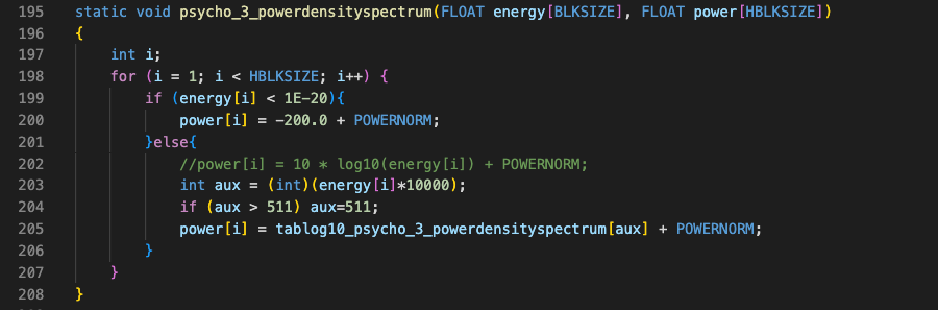
\includegraphics[width=0.80\linewidth]{powerdensityspectrum.pdf}}}
\caption{\textit{psycho\_3\_powerdensityspectrum} function.}
\label{powerdensityspectrum}
\end{figure}
\end{comment}

%\vspace{1cm}

The second case was \textit{psycho\_3\_init\_add\_db}, also in \textit{psycho\_3.c}. In this function, there were both \textit{pow} and \textit{log10} operations inside a \textit{i} loop, with \textit{i} ranging from 0 to 999 (DBTAB-1). However, this case was straightforward to solve, since the result produced in each iteration does not depend on any input data. Considering this, the \textit{tablog10\_psycho\_3\_init\_add\_db} was created by calculating the whole expression in an excel sheet, with \textit{x} ranging from 0 to 99.9 ($x=i/10.0$).

\begin{comment}
\begin{figure}[H]
\centerline{\fbox{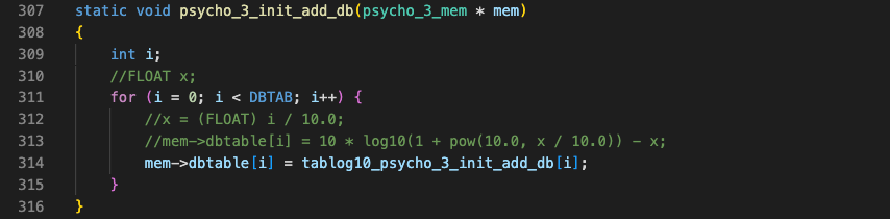
\includegraphics[width=0.80\linewidth]{init.pdf}}}
\caption{\textit{psycho\_3\_init\_add\_db} function.}
\label{init}
\end{figure}
\end{comment}

%\vspace{1cm}

The third case was \textit{psycho\_3\_spl}, in \textit{psycho\_3.c}. In this function, there was a \textit{log10} operation inside a \textit{i} loop, with \textit{i} ranging from 0 to 31 (SBLIMIT-1). Since the \textit{log10} operation was performed based on \textit{scale[i]} and its value was never higher than 20000 (after being multiplied by 32768), the solution was creating a table with 2000 positions, so that \textit{scale[i]} determines the index that should be accessed from the table. 
To be linear access, \textit{scale[i]} has to be multiplied by 3276.8 and converted to an integer. Since it is guaranteed that the array value is always positive, a condition was added to limit the index of the log10 table (1999 is the maximum index). With this, and noticing the multiplication by 20 followed by the subtraction by 10 (of log10) in the original code, the \textit{tablog10\_psycho\_3\_spl} was created by calculating $20\times log10(x\times 10)-10$ in an excel sheet, with \textit{x} ranging from 0 and 1999. It was then copied and defined in \textit{psycho\_3.c}.

\begin{comment}
\begin{figure}[H]
\centerline{\fbox{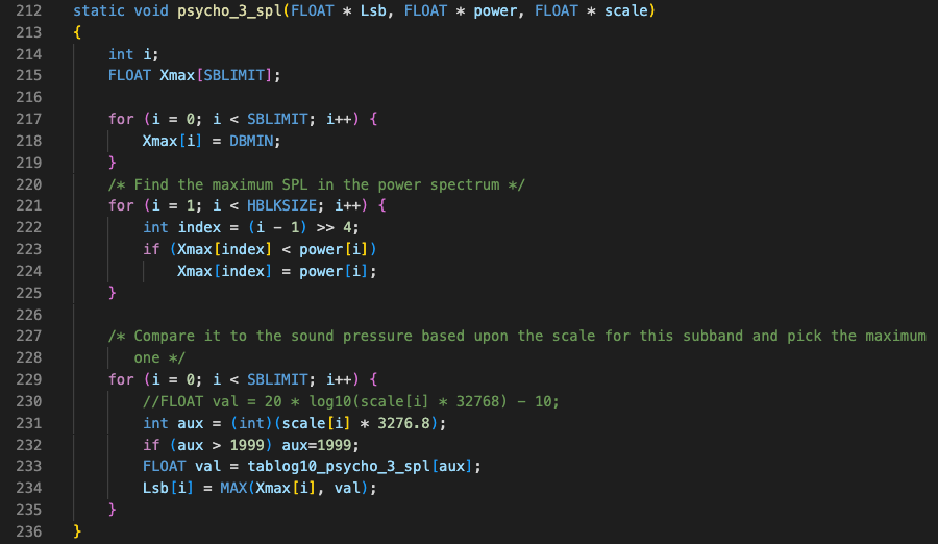
\includegraphics[width=0.80\linewidth]{spl.pdf}}}
\caption{\textit{psycho\_3\_spl} function.}
\label{spl}
\end{figure}

\vspace{1cm}
\end{comment}

The fourth case was \textit{psycho\_3\_fft}, in \textit{psycho\_3.c} too. In this function, there was a \textit{pow} operation and also a \textit{cos} operation inside a \textit{i} loop, with \textit{i} ranging from 0 to 1023 (BLKSIZE-1). This case was straightforward to solve since the result produced in each iteration does not depend on any input data. Considering this, the \textit{tabcos\_psycho\_3\_fft} was created by calculating both expressions in an Excel sheet, with \textit{x} ranging from 0 to 1023.

\begin{comment}
\begin{figure}[H]
\centerline{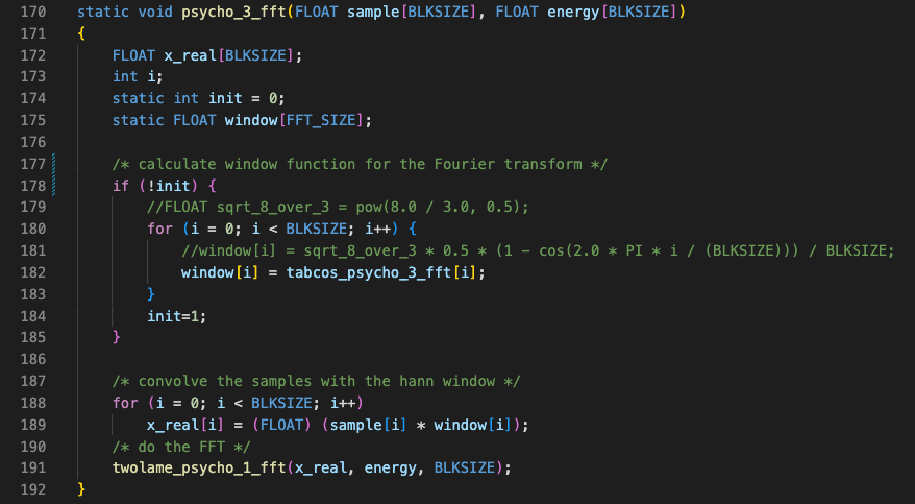
\includegraphics[width=0.80\linewidth]{fft.pdf}}
\caption{\textit{psycho\_3\_fft} function.}
\label{fft}
\end{figure}

\vspace{1cm}
\end{comment}

The fifth and last case was \textit{create\_dct\_matrix}, in \textit{subband.c}. In this function, there was a \textit{cos} operation inside a nested loop, with \textit{i} ranging from 0 to 15 and \textit{k} ranging from 0 to 31. This case was also straightforward to solve since the result produced in each iteration does not depend on any input data. Considering this, the \textit{tabcos\_create\_dct\_matrix} was created by calculating the whole expression in an Excel sheet, with \textit{aux} ranging from 0 to 511 ($16 \times 32$).

\begin{comment}
\begin{figure}[H]
\centerline{\fbox{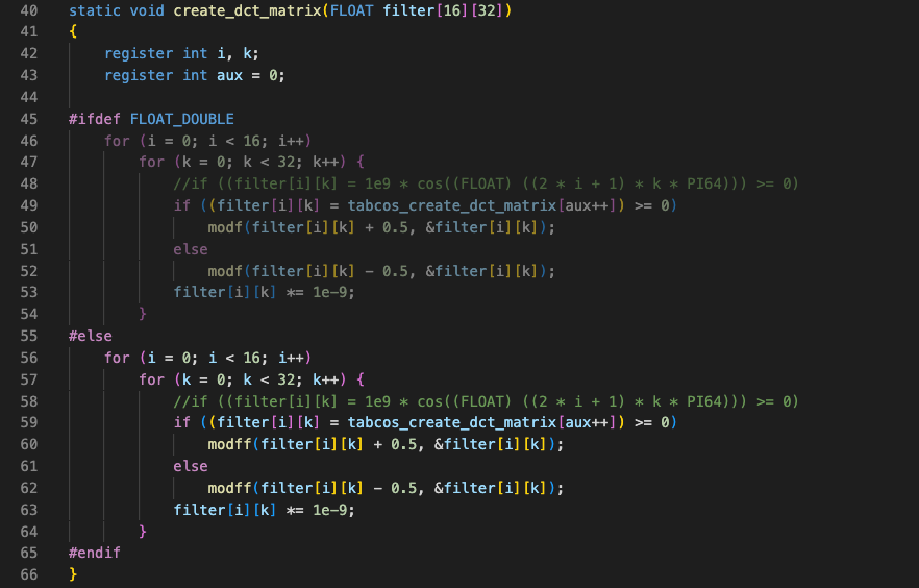
\includegraphics[width=0.80\linewidth]{dct.pdf}}}
\caption{\textit{create\_dct\_matrix} function.}
\label{dct}
\end{figure}

\vspace{1cm}
\end{comment}

The third and last change in \textit{libtwolame} was related to memory.
Initially, there was a memory allocation for \textit{bit\_stream} struct in \textit{twolame\_buffer\_init}, called from \textit{twolame\_encode\_buffer\_interleaved} function. Since this function executes in every \textit{while} loop iteration, in \textit{firmware.c}, the memory allocation was also performed many times.
Therefore, the \textit{TWOLAME\_MALLOC} of \textit{bit\_stream} struct was moved to the \textit{main} function, meaning that it executes just once before the encoding process starts.
In addition, the \textit{TWOLAME\_FREE} in \textit{twolame\_buffer\_deinit}, called from \textit{twolame\_encode\_buffer\_interleaved}, was removed and, consequently, added to \textit{main}. 
After this process, the system was emulated on the PC once again to check correctness.

With basic software optimizations already implemented, the next move was measuring the execution time of IOb-MP2-E in FPGA, for different input data. 
This requires different memory management since allocating memory during program execution on an FPGA can be less straightforward than on a traditional CPU or software-based system. In an FPGA, memory allocation typically needs to be done statically, rather than dynamically during program execution. FPGA-based systems, like IOb-MP2-E, are designed to have a fixed memory structure, and memory is allocated during the configuration of the FPGA (which is static once it is programmed) rather than at runtime. 
That said, there are some scenarios where dynamic memory allocation is possible on an FPGA, in case they provide memory blocks that can be accessed and reconfigured during runtime, but this is usually limited in capacity and not that flexible.

Considering this, a macro called \textit{PC\_EMUL\_RUN} is defined to control each memory allocation, through an if directive. In the first case when the program is emulated on PC, \textit{PC\_EMUL\_RUN} should be defined. In a second case when the program runs in FPGA, \textit{PC\_EMUL\_RUN} should not be defined.
Focusing on the second case, the memory space available starts at \textit{DATA\_BASE\_ADDR}. This macro defines the base address based on IOb-MP2-E macros from \textit{config.mk}, the IOb-MP2-E configuration script.
In \textit{main()}, the first example is \textit{recvfile\_ch} pointer, which represents where the input data is stored in memory. As it is the first, it should be equal to \textit{DATA\_BASE\_ADDR}.
The second example is \textit{pcmaudio} pointer, which represents where the input data buffer is stored. As it is the second, it should be equal to DATA\_BASE\_ADDR + recv\_file\_size (the size of the input file).
The third example is \textit{mp2buffer} pointer, which represents where the encoded data buffer is stored. It should be equal to $pcmaudio + AUDIObUFSIZE*sizeof(short)$ (the second pointer plus the size of the input data buffer).
The fourth example is \textit{mybs} pointer, which represents where the bit\_stream struct is stored. It should be equal to $mp2buffer + MP2BUFSIZE*sizeof(unsigned char)$ (the third pointer plus the size of the encoded data buffer).
The fifth and last example is \textit{outfile} pointer, which represents where the encoded MP2 data is stored. It should be equal to $mybs + sizeof(bit\_stream)$ (the fourth pointer plus the size of the \textit{bit\_stream} struct).
In addition, the \textit{free()} functions were also inserted in a \textit{\#ifdef PC\_EMUL\_RUN} directive, since the function should only be called when the memory is dynamically allocated.  

\subsection{Profiling}

The last implementation in the software architecture was \textbf{profiling}~\cite{profiling}. This process is a form of dynamic program analysis that can measure different variables, like memory space or time complexity. In this case, it was used to measure the duration of each function.
The process of profiling \textit{TwoLAME} consisted of three phases, with the first phase being a more high-level approach. 
This phase was simple since only the function calls directly made from \textit{main()} were considered. The timer was first initialized through \textit{timer\_init(TIMER\_BASE)} function. Then, a \textit{elapsed\_time} integer array of size 50 was declared and set with zero. In the profiling itself, some basic operations were used for each function call. Immediately before a function call, \textit{timer\_time\_ms()} is invoked, returning the current time in ms which is then stored in \textit{start\_elapse\_time} variable as an unsigned integer. Immediately after a function call, \textit{timer\_time\_ms()} is invoked again, returning the current time in ms which is then stored in \textit{end\_elapse\_time} variable as an unsigned integer as well. Then, the difference between both variables is calculated and stored in a certain index of \textit{elapsed\_time} array (one index for each function call). 
By doing this, 13 functions were included in the first phase of \textit{TwoLAME} profiling. At the end of \textit{main()}, every position of the array is printed, showing how many ms each function call took. The printing does not influence the profiling, as it is done after the last function measurement. Another interesting detail is that both \textit{uart\_recvfile} and \textit{uart\_sendfile} functions are excluded from the profiling, which is correct since they perform data transfers that are not part of the \textit{TwoLAME}.
Table \ref{profiling1} shows the first phase of the profiling for all input files, presented in \textit{Results} section.

By analyzing \textit{twolame\_encode\_buffer\_interleaved}, it is noticeable that the relevant operation inside the function is \textit{encode\_frame()}, as all the other are basic.
Considering this, the second phase of profiling includes all function calls inside \textit{encode\_frame}. 
This phase was similar to the previous one in terms of methodology. The only differences were the usage of the \textit{elapsed\_time\_twolame} array, which was declared and set to 0 in \textit{main()} and passed as an argument to \textit{twolame\_encode\_buffer\_interleaved} and \textit{encode\_frame()}, consecutively. The variables that store the time values are also different, being \textit{start\_elapse\_time\_twolame} and \textit{end\_elapse\_time\_twolame}, declared in \textit{twolame.c} as global unsigned integers.
By doing this, 23 functions were included in the second phase of \textit{TwoLAME} profiling. It was not 23 functions but 23 blocks of code from \textit{encode\_frame()}, because apart from the \textit{libtwolame} functions, there is additional code that has to be included for correct measurements, like if conditions and \textit{for} loops.
At the end of \textit{main()}, every position of the array is printed, showing how many ms each part of \textit{encode\_frame()} took. 
Table \ref{profiling2} shows the second phase of the profiling for all input files, , presented in \textit{Results} section.

Looking at \textit{twolame\_psycho\_3}, there are many other \textit{libtwolame} functions inside it. Considering this, the third phase of profiling includes all function calls inside \textit{twolame\_psycho\_3}. 
This phase was also similar to the previous ones in terms of methodology. The only differences were the usage of the \textit{elapsed\_time\_psycho\_3} array, which was declared and set to 0 in \textit{main()} and passed as argument to \textit{twolame\_encode\_buffer\_interleaved}, \textit{encode\_frame()} and \textit{twolame\_psycho\_3}, consecutively. The variables that stored the time values were also different, being \textit{start\_elapse\_time\_psycho\_3} and \\ \textit{end\_elapse\_time\_psycho\_3}, declared in \textit{twolame.c} as global unsigned integers.
By doing this, 13 blocks of code were included in the third phase of \textit{TwoLAME} profiling, with most of them being just functions.
At the end of \textit{main()}, every position of the array is printed, showing how many ms each block of \textit{twolame\_psycho\_3} took. 
Table \ref{profiling3} shows the third phase of the profiling for all input files, presented in \textit{Results} section.


%These functions have more specific names as we are going lower in abstraction.